\dev{Bertrand Jules}{\cite{Robert}}

\textit{
Ce développement propose un algorithme d'approximation pour un problème d'ordonnancement de tâches indépendantes. Ainsi, il s'intègre dans les leçons \ref{L11} et \ref{L13}. 
Cet algorithme étant glouton, il illustre aussi cette stratégie pour la leçon \ref{L12}.
}

\paragraph{Problème.} On considère le problème d’ordonnancement suivant.

\begin{definition}[$\mathbf{INDEP}(p)$]~

\noindent \textbf{Données} : n tâches $\{T_1,...,T_n\}$ et $p\geq 2$ processeurs. À chaque tâche $T_i$ est associée un poids $w(T_i)$.

\noindent \textbf{Sortie} : ordonnancement des tâches $\mathbf{alloc} :  \{T_1,...,T_n\} \rightarrow \{1,...,p\}$, tel que 
$$
\max_{1\leq l \leq p} \sum_{T_i \in \mathbf{alloc}^{-1}(l)}w(T_i)
$$
soit minimal.
\end{definition}


\begin{example} On prend 4 tâches, avec $w(T_1)=2$, $w(T_2)=2$, $w(T_3)=3$.

\begin{center}
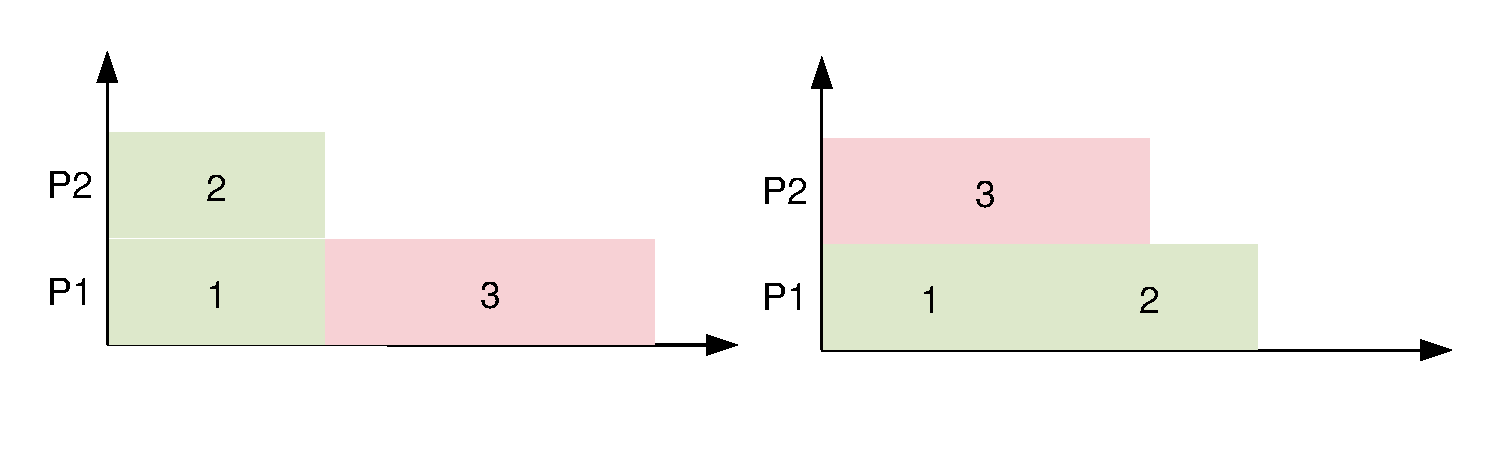
\includegraphics[scale=0.6]{Developpements/Approximation ordonnancement/exemple1.pdf} 
\end{center}
\end{example}

On considère l'algorithme \textbf{glouton-online} qui, pour toute tâche $T_1,...,T_n$, l'affecte au processeur le plus libre. Sur l'exemple précédent, l'ordonnancement obtenu via \textbf{glouton-online} correspond au schéma de gauche. On remarque directement que cet algorithme n'est pas optimal.

\begin{theorem}[Résultat d'approximation]~

\textbf{glouton-online} est une $\left(2-\frac{1}{p}\right)$-approximation pour le problème $\mathbf{INDEP}(p)$. Le facteur d'approximation est atteint.
\end{theorem}

\paragraph{Notations.} On note $\tau^*$ le temps d'exécution optimal d'un ordonnancement de ces tâches et $S=\sum_{i=1}^n w(T_i)$. 

\begin{lemma}
$\tau^* \geq \frac{1}{p}\sum_{i=1}^n w(T_i)$
\end{lemma}

\begin{proof}
On note $\tau_1,...,\tau_p$ les temps d'exécutions sur chaque processeur, et on a alors $ S := \sum_{i=1}^n w(T_i) = \sum_{k=1}^p \tau_k$.

On sait que $\tau^* = \max_{1\leq k\leq p} \tau_k$. Ainsi, 
$$
S \leq \sum_{k=1}^p \tau^*
$$
La lemme en découle directement.
\end{proof}

\paragraph{Preuve du théorème.} On suppose que l'algorithme \textbf{glouton-online} retourne un ordonnancement $\mathbf{alloc}$ de nos $n$ tâches, de temps d'exécution total $\tau$. On veut montrer que 
$$
\frac{\tau}{\tau^*}\leq 2-\frac{1}{p}
$$

On suppose sans perdre de généralité que $\tau=\tau_1$, c'est-à-dire que c'est le premier processeur qui termine en dernier. On note $T_j$ la dernière tâche exécutée sur $P_1$, et on note $\tau_0=\tau_1 -w(T_j)$, c'est-à-dire le temps d'exécution avant qu'on affecte $T_j$ à $P_1$. 

On remarque alors que pour tout $2\leq i \leq p$, $\tau_0 \leq \tau_i$. En, effet, s'il existe $2\leq i \leq p$ tel que $\tau_0 >\tau_i$, alors la tâche $T_j$ n'aurait pas été affecté à $P_1$.\newline 

\begin{center}
\textit{Il sera judicieux d'illustrer avec un schéma sur lequel apparaît $T_j$, $\tau_0$ et $\tau_1$.}
\end{center}

\begin{align*}
S &= \sum_{i=1}^p \tau_i \\
&= \tau_1 + \sum_{i=2}^p \tau_i \\
&\geq \tau_1 + (p-1)\tau_0 \\ 
&= p \tau_1 - (p-1) w(T_j) \\
&= p\tau -(p-1)w(T_j)
\end{align*} 

Or, on remarque que $w(T_j) \leq \tau^*$, et par le lemme précédent, $\tau^* \geq \frac{1}{p}S$. Ainsi, 
$$
\tau \leq \frac{S}{p} + \frac{p-1}{p} w(T_j) \leq \tau^* +\frac{p-1}{p} \tau^* = \left(2- \frac{1}{p}\right) \tau^*
$$

Montrons que le facteur est atteint. Pour cela on considère $p(p-1)$ tâches de taille $1$ et une tâche de taille $p$. La solution optimale consiste à affecter la tache de taille $p$ à un processeur, et $p$ tâches de taille $1$ aux $p-1$ processeurs restants. On obtient $\tau^*=p$.

La solution gloutonne qui prend la grande tâche en dernier va alors remplir les $p$ processeurs de manière équilibrée avec les $p(p-1)$ premières tâches. Ainsi, lorsqu'on affecte la dernière tâche, tous les processeurs sont remplis avec $p-1$ tâches et ainsi $\tau=p-1+p=2p-1$. Finalement, 
$$
\frac{\tau}{\tau^*} = \frac{2p-1}{p}= 2 -\frac{1}{p}
$$

\begin{center}
\textit{ On pourra mentionner le fait que l'algorithme glouton offline, qui trie les tâches avant de les exécuter n'est pas optimal non plus, mais donne un meilleur facteur d'approximation.}
\end{center}